\section{Hyperparameter Exploration}

\subsection{Experiment: Deeper CNN (Option B)}

\textbf{Architecture:} Added a third convolutional layer (64 channels) with MaxPooling to the original CNN.

\begin{itemize}
    \item Validation accuracy: \textbf{99.29\%}
    \item Number of parameters: \textbf{458,570}
    \item Training epochs: \textbf{20}
\end{itemize}

\begin{figure}[h]
    \centering
    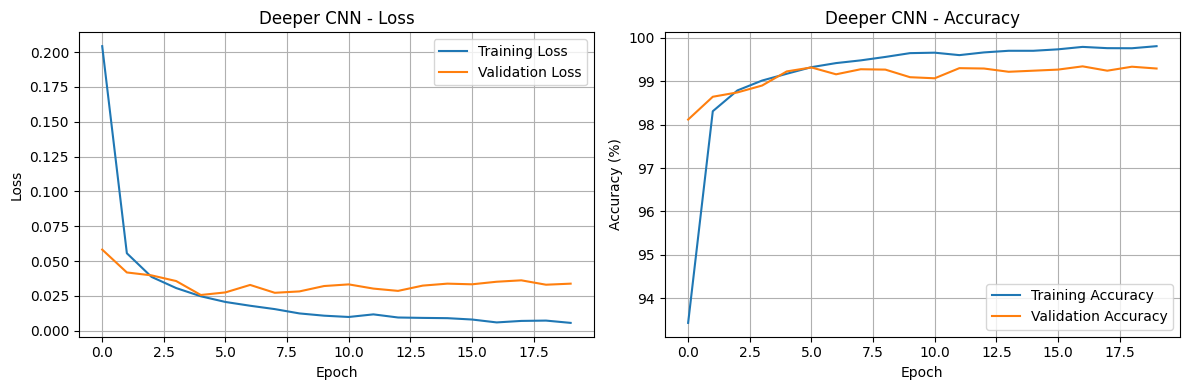
\includegraphics[width=0.7\linewidth]{section4/deeper_cnn.png}
    \caption{Training and validation curves for Deeper CNN}
    \label{fig:deeper-cnn}
\end{figure}

\textbf{Performance Analysis:} The deeper CNN achieved 99.29\% validation accuracy compared to 99.03\% for the original CNN. An improvement of only 0.26\% despite an 8.8\% increase in parameters (36,928 additional). This minimal improvement demonstrates diminishing returns: the 2-layer CNN was already near-optimal for MNIST's complexity.

\subsection{Learning Rate Sensitivity Experiment}

Testing with $\text{learning rate} = 0.1$ (100× larger than optimal 0.001):

\begin{figure}[h]
    \centering
    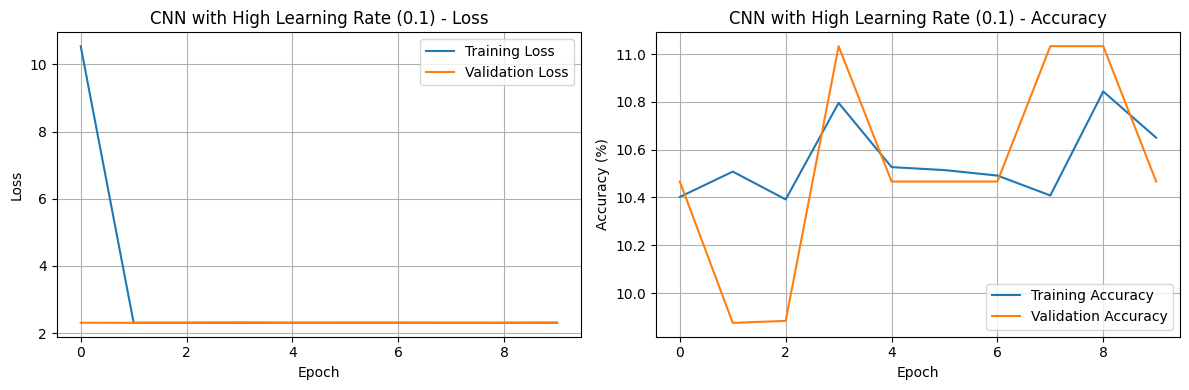
\includegraphics[width=0.7\linewidth]{section4/high_lr.png}
    \caption{Training instability with high learning rate (0.1)}
    \label{fig:high-lr}
\end{figure}

\begin{table}[h]
\centering
\begin{tabular}{|l|c|c|}
\hline
\textbf{Learning Rate} & \textbf{Val Accuracy} & \textbf{Training Loss} \\ \hline
0.001 (normal) & 99.2\% & 0.23 \\ \hline
0.1 (high) & 10.5\% & 10.54 \\ \hline
\end{tabular}
\caption{Impact of excessive learning rate}
\label{tab:lr-comparison}
\end{table}

\subsubsection{Question 4.2: What happened with high learning rate?}

Training with $LR=0.1$ resulted in complete failure, achieving only 10.5\% validation accuracy (barely above random guessing). The learning rate controls step size in gradient descent: $w_{new} = w_{old} - \alpha \cdot \nabla L$. A 100× larger learning rate causes:

\begin{itemize}
    \item \textbf{Overshooting}: Steps too large to converge; the model bounces around the loss landscape instead of settling into a minimum
    \item \textbf{Instability}: Weight updates are massive, preventing the model from learning meaningful features
    \item \textbf{Loss explosion}: Training loss fluctuates wildly (around 2.3-10.54) with no downward trend
\end{itemize}

This demonstrates that learning rate is one of the most critical hyperparameters, even advanced optimizers like Adam cannot compensate for grossly inappropriate values.